\documentclass[english,10pt,aspectratio=169]{beamer}

\usepackage{amsmath}
\usepackage[T1]{fontenc}
\usepackage{listings}
\usepackage{tikz}
\usepackage{ulem}

%%%%%%%%%%%%%%%%%%%%%%%%%%%%%%%%%%%%%%%%%%%%%%%%%%%%%%%%%%%
% beamer
%%%%%%%%%%%%%%%%%%%%%%%%%%%%%%%%%%%%%%%%%%%%%%%%%%%%%%%%%%%
\mode<presentation>
\usetheme{singapore}
\usecolortheme{orchid}

%%%%%%%%%%%%%%%%%%%%%%%%%%%%%%%%%%%%%%%%%%%%%%%%%%%%%%%%%%%
% listings
%%%%%%%%%%%%%%%%%%%%%%%%%%%%%%%%%%%%%%%%%%%%%%%%%%%%%%%%%%%
\lstdefinestyle{PythonStyle}{
	basicstyle=\scriptsize\ttfamily,
	language=Python,
	numbers=left,
	tabsize=4
}
\lstset{basicstyle=\small,style=PythonStyle}

%%%%%%%%%%%%%%%%%%%%%%%%%%%%%%%%%%%%%%%%%%%%%%%%%%%%%%%%%%%
% tikz
%%%%%%%%%%%%%%%%%%%%%%%%%%%%%%%%%%%%%%%%%%%%%%%%%%%%%%%%%%%
\usetikzlibrary{shapes.geometric, arrows}
\tikzstyle{startstop} = [
	rectangle,
	rounded corners,
	minimum width=1cm,
	minimum height=0.5cm,
	text centered,
	draw=black,
	fill=red!30
]
\tikzstyle{io} = [
	trapezium,
	trapezium left angle=70,
	trapezium right angle=110,
	minimum width=1cm,
	minimum height=0.5cm,
	text centered,
	draw=black,
	fill=blue!30
]
\tikzstyle{process} = [
	rectangle,
	minimum width=1cm,
	minimum height=0.5cm,
	text centered,
	draw=black,
	fill=orange!30
]
\tikzstyle{decision} = [
	diamond,
	minimum width=1cm,
	minimum height=0.5cm,
	text centered,
	draw=black,
	fill=green!30
]
\tikzstyle{arrow} = [thick, ->, >=stealth]
%%%%%%%%%%%%%%%%%%%%%%%%%%%%%%%%%%%%%%%%%%%%%%%%%%%%%%%%%%%
% commands
%%%%%%%%%%%%%%%%%%%%%%%%%%%%%%%%%%%%%%%%%%%%%%%%%%%%%%%%%%%
\newcommand{\focus}[1]{\textcolor{blue}{#1}}

\newcommand{\hideit}[1]{%
  \only<0| handout:1>{\mbox{}}%
  \invisible<0| handout:1>{#1}%
}

\def\presentationtitle{\textbf{
  Spending less time bug fixing by \\
  spending more time unit testing
}}

\title{\large\presentationtitle}
\author{\textbf{
  <Name>
}}
\date{}

\begin{document}

%%%%%%%%%%%%%%%%%%%%%%%%%%%%%%%%%%%%%%%%%%%%%%%%%%%%%%%%%%%
% code listings 
%%%%%%%%%%%%%%%%%%%%%%%%%%%%%%%%%%%%%%%%%%%%%%%%%%%%%%%%%%%
\defverbatim[colored]\coveragecode{%
\begin{lstlisting}[linewidth=0.5\textwidth]
def is_fizzbuzz(num: int) -> bool:
    if num % 3 and num % 5:
        return True
    return some_var

def test_fizzbuzz():
    result = is_fizzbuzz(3)
    assert result
\end{lstlisting}
}

\defverbatim[colored]\coveragecodetwo{%
\begin{lstlisting}[linewidth=0.5\textwidth]
def is_fizzbuzz(num: int) -> bool:
    return True if num % 3 and num % 5 else some_var

def test_fizzbuzz():
    result = is_fizzbuzz(3)
    assert result
\end{lstlisting}
}

\defverbatim[colored]\coveragecodebranch{%
\begin{lstlisting}[linewidth=0.5\textwidth]
def generate_number(
    cond_1: bool = True,
    cond_2: bool = True,
    cond_3: bool = True,
) -> int:
    if cond_1:
        num = 1
    if cond_2:
        num = 2
    if cond_3:
        num = 3
    return num
\end{lstlisting}
}


\begin{frame}
  \titlepage
\end{frame}

% To begin with a quote from the author, "There's much more to unit testing than
% the act of writing tests." Hopefully this presentation will be able to get you
% to think more about how to craft unit tests.
\begin{frame}
  \begin{quote}
    There's much more to unit testing than the act of writing tests.
    \begin{flushright}
      \tiny{---Khorikov, \textup{Unit Testing Principles, Practices, and Patterns}, 3}
    \end{flushright}
  \end{quote}
\end{frame}

% The goal of unit testing is to enable sustainable growth of the software
% project. The figure below show the growth dynamics of a typical project without
% tests. You start off quick, completing user stories after user stories, without
% having to "waste" writing these pesky tests.
% But eventually progress slows to a halt, the code base has grown complex and
% disorganized, fixing one bug introduces several others, and changing one part
% of the software breaks several others. And it's hard to bring it back to
% stability.
% This is where tests help, they help detect regressions and ensure existing
% functionalities work even after refactoring or introducing new features.
\begin{frame}{The goal of unit testing}
  To enable \textbf{sustainable} growth of software project.
  \begin{columns}[T]
    \begin{column}{0.5\textwidth}
      \includegraphics[width=\textwidth]{images/vs_no_test.png}
    \end{column}
    \begin{column}{0.5\textwidth}
    \end{column}
  \end{columns}
\end{frame}

% But it's not enough to just write tests. Badly written tests still result in
% the same picture. They help slow down the initial decline in development speed
% but doesn't really change much overall. Before we look at what makes a good unit
% test, let's first look at code coverage metrics which can help you gauge if you
% are testing enough.
\begin{frame}{The goal of unit testing}
  To enable \textbf{sustainable} growth of software project.
  \begin{columns}[T]
    \begin{column}{0.5\textwidth}
      \includegraphics[width=\textwidth]{images/vs_no_test.png}
    \end{column}
    \begin{column}{0.5\textwidth}
      \includegraphics[width=\textwidth]{images/vs_bad_test.png}
    \end{column}
  \end{columns}
\end{frame}

% The common belief is that the higher the coverage number, the better the test
% suite. Unfortunately, it's not that simple. While 10% is a good indication
% that you aren't testing enough, 100% coverage doesn't guarantee you have a
% good quality test suite. We take a look at a few coverage metrics to see why
% this is so.
% We will discuss 4 types of coverage metrics. Path and condition coverage are
% struck out because while they're nice to think about, they're impractical to
% actually implement.
% < describe the code and coverage stats > 
\begin{frame}{Coverage metrics}
  \focus{Statement} vs Branch vs \sout{Path} vs \sout{Condition}
  \begin{columns}[T]
    \begin{column}[]{0.6\textwidth}
      \begin{minipage}{\linewidth}
        \coveragecode
      \end{minipage}
    \end{column}
    \begin{column}[]{0.4\textwidth}
      \begin{flalign*}
        &\frac{Number\ of\ statements\ executed}{Total\ number\ of\ statements}\\
        \approx\ &67 \%
      \end{flalign*}
    \end{column}
  \end{columns}
\end{frame}

% One simple trick to improve our statement coverage metric to refactor the
% function into a conditional expression. Now we get 100% statement coverage
% without having to write any extra tests. This just shows how easy it is to game
% the coverage metrics.
\begin{frame}{Coverage metrics}
  \focus{Statement} vs Branch vs \sout{Path} vs \sout{Condition}
  \begin{columns}[T]
    \begin{column}[]{0.6\textwidth}
      \begin{minipage}{\linewidth}
        \coveragecodetwo
      \end{minipage}
    \end{column}
    \begin{column}[]{0.4\textwidth}
      \begin{flalign*}
        &\frac{Number\ of\ statements\ executed}{Total\ number\ of\ statements}\\
        =\ &100 \%
      \end{flalign*}
    \end{column}
  \end{columns}
\end{frame}

% Branch coverage considers how many control structures are traversed by at least
% one test in the test suite. And reports 50% coverage no matter how we refactor
% the function.
\begin{frame}{Coverage metrics}
  Statement vs \focus{Branch} vs \sout{Path} vs \sout{Condition}
  \begin{columns}[T]
    \begin{column}[]{0.6\textwidth}
      \begin{minipage}{\linewidth}
        \coveragecodetwo
      \end{minipage}
    \end{column}
    \begin{column}[]{0.4\textwidth}
      \begin{flalign*}
        &\frac{Branches\ traversed}{Total\ number\ of\ branches}\\
        =\ &50 \%
      \end{flalign*}
    \end{column}
  \end{columns}
\end{frame}

% To help visualize this metric, the flowchart shows the possible paths of the
% function. And the test_fizzbuzz() function only traversed through one of them.
\begin{frame}{Coverage metrics}
  Statement vs \focus{Branch} vs \sout{Path} vs \sout{Condition}
  \begin{columns}[T]
    \begin{column}[]{0.6\textwidth}
      \begin{minipage}{\linewidth}
        \coveragecodetwo
      \end{minipage}
    \end{column}
    \begin{column}[]{0.4\textwidth}
      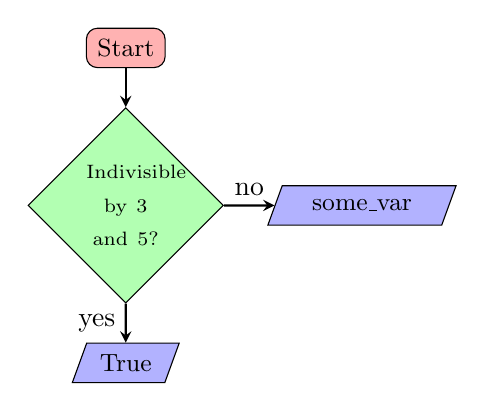
\begin{tikzpicture}[node distance=2cm]
        \node (start) [startstop] {\small{Start}};
        \node (decision)
          [decision, below of=start, text width=1cm, align=center]
          {\scriptsize{Indivisible by 3 and 5?}};
        \node (out1) [io, below of=decision] {\small{True}};
        \node (out2) [io, right of=decision, xshift=1cm] {\small{some\_var}};
        \draw [arrow] (start) -- (decision);
        \draw [arrow] (decision) -- node[anchor=east] {yes} (out1);
        \draw [arrow] (decision) -- node[anchor=south] {no} (out2);
      \end{tikzpicture}
    \end{column}
  \end{columns}
\end{frame}

% This function has 3 if conditions each returning a different number. Branch
% coverage requires 6 test cases. But does achieving 100% branch coverage
% ensure that this function won't crash? What happens when all 3 conditions
% evaluate to False? Path coverage ensures all paths are covered. It will test
% path BDF and catch the bug. Although this will give you a very comprehensive
% coverage of your code, 100% path coverage is impractical to aim for in reality.
\begin{frame}{Coverage metrics}
  Statement vs Branch vs \focus{\sout{Path}} vs \sout{Condition}
  \begin{columns}[T]
    \begin{column}[]{0.5\textwidth}
      \begin{minipage}{\linewidth}
        \coveragecodebranch
        Possible paths:

        ACE, ACF, ADE, ADF, BCE, BCF, BDE, BDF
      \end{minipage}
    \end{column}
    \begin{column}[]{0.5\textwidth}
      \begin{tikzpicture}[node distance=1.3cm]
        \node (start) [startstop] {\small{Start}};
        \node (dec1) [decision, below of=start, aspect=3, yshift=1mm]
          {\scriptsize{cond\_1?}};
        \node (out11) [io, left of=dec1, xshift=-1.75cm, label={A}]
          {\small{num = 1}};
        \node (out12) [io, right of=dec1, xshift=1cm, label={B}] {\small{pass}};
        \node (dec2) [decision, below of=dec1, aspect=3]
          {\scriptsize{cond\_2?}};
        \node (out21) [io, left of=dec2, xshift=-1.75cm, label={C}]
          {\small{num = 2}};
        \node (out22) [io, right of=dec2, xshift=1cm, label={D}] {\small{pass}};
        \node (dec3) [decision, below of=dec2, aspect=3]
          {\scriptsize{cond\_3?}};
        \node (out31) [io, left of=dec3, xshift=-1.75cm, label={E}]
          {\small{num = 3}};
        \node (out32) [io, right of=dec3, xshift=1cm, label={F}] {\small{pass}};
        \node (end) [startstop, below of=dec3] {\small{End}};
        \draw [arrow] (start) -- (decision);
        \draw [arrow] (dec1) -- node[anchor=south] {yes} (out11);
        \draw [arrow] (dec1) -- node[anchor=south] {no} (out12);
        \draw [arrow] (out11) |- ++(0, -5mm) -| (dec2);
        \draw [arrow] (out12) |- ++(0, -5mm) -| (dec2);
        \draw [arrow] (dec2) -- node[anchor=south] {yes} (out21);
        \draw [arrow] (dec2) -- node[anchor=south] {no} (out22);
        \draw [arrow] (out21) |- ++(0, -5mm) -| (dec3);
        \draw [arrow] (out22) |- ++(0, -5mm) -| (dec3);
        \draw [arrow] (dec3) -- node[anchor=south] {yes} (out31);
        \draw [arrow] (dec3) -- node[anchor=south] {no} (out32);
        \draw [arrow] (out31) |- ++(0, -5mm) -| (end);
        \draw [arrow] (out32) |- ++(0, -5mm) -| (end);
      \end{tikzpicture}
    \end{column}
  \end{columns}
\end{frame}

% The goal of condition coverage is to check individual outcomes for each logical
% condition. Branch coverage requires only 2 test cases, but condition coverage
% requires 4. Aiming for 100% conditional coverage is also impractical.
% Say, a test suite achieved 100% on all coverage metrics for this is_fizzbuzz()
% function, does that mean the test suite is guaranteed to cover all use cases
% catch all bugs? What if the user supplies a string instead of a int?
\begin{frame}{Coverage metrics}
  Statement vs Branch vs \sout{Path} vs \focus{\sout{Condition}}
  \begin{columns}[T]
    \begin{column}[]{0.5\textwidth}
      \begin{minipage}{\linewidth}
        \coveragecode
      \end{minipage}
    \end{column}
    \begin{column}[]{0.5\textwidth}
      \begin{center}
        \begin{tabular}{ ccc }
          \hline
          \texttt{num \% 3} & \texttt{num \% 5} & \texttt{num \% 3 and num \% 5} \\
          \hline
          True & True & True \\
          True & False & False \\
          False & True & False \\
          False & False & False \\
          \hline
        \end{tabular}
      \end{center}
    \end{column}
  \end{columns}
\end{frame}

\begin{frame}
  \begin{quote}
    [C]overage metrics are a good negative indicator, but a bad positive one.
    \begin{flushright}
      \tiny{---Khorikov, \textup{Unit Testing Principles, Practices, and Patterns}, 15}
    \end{flushright}
  \end{quote}
\end{frame}
\end{document}
